\documentclass[a4paper]{article}
%The main tex begins from line 262
\usepackage[top = 2.5cm, bottom = 2.5cm, left = 2cm, right = 2cm]{geometry} 
\usepackage{amsmath} % For the usage of \because and \therefore
\usepackage{amssymb}
\usepackage{fancyhdr}
\usepackage{lastpage}
\usepackage{etoolbox}
\usepackage{indentfirst}
\usepackage{tabularx}
\usepackage{mathtools}
\usepackage{booktabs}
\usepackage{authblk}
\usepackage[calcwidth]{titlesec}
\usepackage{bookmark}
\usepackage[capitalize]{cleveref}
\usepackage{array}
\usepackage[english]{babel}
\usepackage{enumitem} % For the usage of labeling in enumerate and itemize
%\usepackage[utf8]{inputenc}
%\usepackage{CJKutf8}
\usepackage{xeCJK}

%%%%%%%%%%%%%%%%%%%%%%%%%%%%%%%%%%%%%%%%%%%%%%%%%%%

\makeatletter
% Macros for setting basic info
\gdef\@uni{National Taiwan University}
\gdef\@department{Information Management}
\gdef\@me{Yu-Chieh Kuo}

\newcommand{\course}[2][]{
    \ifstrempty{#1}{
        \gdef\shortcourse{#2}
    }{
        \gdef\shortcourse{#1}
    }
    \gdef\@course{#2}
}
\newcommand{\teacher}[1]{\gdef\@teacher{#1}}
\newcommand{\semester}[1]{\gdef\@semester{#1}}
\newcommand{\uni}[1]{\gdef\@uni{#1}}
\newcommand{\department}[1]{\gdef\@department{#1}}
\newcommand{\student}[3][]{
    \ifstrempty{#1}{
        \author{\textbf{#2} \textbf{#3}}
    }{
        \author[#1]{\textbf{#2} \textbf{#3}}
    }
}
\newcommand{\assignment}[2][Homework]{
    \ifstrempty{#2}{
        \gdef\@assignment{#1}
    }{
        \gdef\@assignment{#1 #2}
    }
}

% page style for title page
\fancypagestyle{title}{
    \fancyhf{}
    \renewcommand{\headrulewidth}{0pt}
    \cfoot{\footnotesize Page {\thepage} of \pageref{LastPage}} 
}
\newcommand{\ujtitle}{
    \thispagestyle{title}
    \noindent\begin{tabularx}{\linewidth}{Xr} % This is a simple tabular environment to align your text nicely 
    {\large \bf{\@course}} \\
    National Taiwan University, \@semester  \\
    \bottomrule % \hline produces horizontal lines.
    \end{tabularx}
    
    \vspace*{0.3cm}

    \begin{center}
        {\huge\bf\textsc{\@assignment}}\\[3mm]
        {\@author}
    \end{center}

    \vspace*{0.3cm}
}
\newcommand{\mymaketitle}{
    \thispagestyle{title}
    \vspace*{-15mm}
    \noindent\begin{tabularx}{\linewidth}{Xr}
                                & \textsl{National Taiwan University} \\
        \large\textbf{\@semester,} & \textsl{Department of \@department}         \\
        \large\textbf{\@course} & \textsl{Prof. \@teacher}\Bstrut\\
        \bottomrule
    \end{tabularx}

    \vspace*{10mm}

    \begin{center}
        {\huge\textsc{\@assignment{}}}\\[6mm]
        {\@author}
    \end{center}

    \vspace*{1cm}
}

% page style for contents
\pagestyle{fancy}
\fancyhf{}
\setlength{\headheight}{13.6pt}
\lhead{\small {\@course}: {\@assignment}}
\rhead{\small {\@me}}
\cfoot{\small {Page {\thepage} of \pageref{LastPage}}} 

% Style for part, section, and subsection
% Part
\titleclass{\part}{straight}
\titleformat{\part}
[display]
{\centering\bfseries}
{\setlength{\titlewidth}{1.5\titlewidth}\large\titleline*[c]{\titlerule[.6pt]}\vspace{3pt}\MakeUppercase{\partname} \thepart}
{0pt}
{\LARGE\itshape}
[{
    \setlength{\titlewidth}{1.5\titlewidth}
    \titleline*[c]{\titlerule*{\mdseries-}}
}]
\titlespacing*{\part}{0pt}{20pt}{20pt}[0pt]

% Problem and subproblem
\setcounter{secnumdepth}{0}
\newcounter{problem}
\newcounter{subproblem}[problem]
\newbool{appendix}
\gdef\problemName{Problem}
\newcommand{\problem}[2][]{
    \setcounter{equation}{0}
    \ifstrempty{#1}{
        \stepcounter{problem}
    }{
        \setcounter{problem}{#1}
    }
    \ifstrempty{#2}{
        \ifbool{appendix}{
            \section{\hspace{-5mm}\problemName{} \Alph{problem}.}
        }{
            \section{\hspace{-5mm}\problemName{} \arabic{problem}}
        }
    }{
        \ifbool{appendix}{
            \section{\hspace{-5mm}\problemName{} \Alpa{problem}: #2}
        }{
            \section{\hspace{-5mm}\problemName{} \arabic{problem}: #2}
        }
    }
}
\newcommand{\subproblem}[2][]{
    \setcounter{equation}{0}
    \ifstrempty{#1}{
        \stepcounter{subproblem}
    }{
        \setcounter{subproblem}{#1}
    }
    \ifstrempty{#2}{
        \ifbool{appendix}{
            \section{\hspace{-2mm}\Alph{problem}.\arabic{subproblem}}
        }{
            \section{\hspace{-2mm}\arabic{problem}.(\alph{subproblem})}
        }
    }{
        \ifbool{appendix}{
            \section{\hspace{-2mm}\Alph{problem}.\arabic{subproblem}. #2}
        }{
            \section{\hspace{-2mm}\arabic{problem}.(\alph{subproblem}) #2}
        }
    }
}

% Appendix
\newcommand{\myAppendix}{
    \setcounter{section}{0}
    \renewcommand{\sectionname}{Appendix}
    \renewcommand{\thesection}{\Alph{section}}
    \renewcommand{\thesubsection}{\Alph{section}.\arabic{subsection}}
    \renewcommand{\perhapscolon}[1]{\perhapsdot{##1}}
}

% Bookmarks
\hypersetup{
    bookmarksnumbered=true
}

% Reference nome for task and subtask
\crefname{section}{\sectionname}{\sectionnamepl}

\makeatother

%%%%%%%%%%%%%%%%%%%%%%%%%%%%%%%%%%%%%%%%%%%%%%%%%%%

% \everymath{\displaystyle} % display all math symbol as DISPLAY MODE

% commands for spacing
\newcommand{\Tstrut}{\rule{0pt}{4mm}}         % = `top' strut
\newcommand{\Bstrut}{\rule[-2mm]{0mm}{0mm}}   % = `bottom' strut

% Paired Delimiters {}, (), []
\providecommand\given{} % so it exists
\newcommand\SetSymbol[1][]{
   \nonscript\,#1\vert \allowbreak \nonscript\,\mathopen{}}
\DeclarePairedDelimiterX\Set[1]{\lbrace}{\rbrace}%
 { \renewcommand\given{\SetSymbol[\delimsize]} #1 }
\DeclarePairedDelimiterX{\Bkt}[1]{[}{]}{#1}
\DeclarePairedDelimiterX{\Paren}[1]{(}{)}{#1}
\DeclarePairedDelimiterX{\Abs}[1]{\lvert}{\rvert}{#1}
\newcommand{\PR}[1]{\Pr\Bkt*{#1}}
\newcommand{\overbar}[1]{\mkern 1.5mu\overline{\mkern-1.5mu#1\mkern-1.5mu}\mkern 1.5mu}

\newcolumntype{D}{>{$(}l<{)$}}
\newcolumntype{R}{>{\displaystyle}r}
\newcolumntype{C}{>{\displaystyle}c}
\newcolumntype{L}{>{\displaystyle}l}

%%%%%%%%%%%%%%%%%%%%%%%%%%%%%%%%%%%%%%%%%%%%%%%%%%%

\usepackage{amsfonts}
\usepackage{amsthm}

%%%%%%%%%%%%%%%%%%%%%%%%%%%%%%%%%%%%%%%%%%%%%%%%%%%

% Declare operator and useful math command
\DeclareMathOperator{\EOp}{\mathbb{E}}
\newcommand{\E}[1]{\ensuremath{\EOp\Bkt*{#1}}}
\newcommand{\R}{\mathbb{R}}
\newcommand{\N}{\mathbb{N}}
\newcommand{\Q}{\mathbb{Q}}
\newcommand{\Z}{\mathbb{Z}}
\newcommand{\PS}[1]{\mathcal{P}(#1)}
\newcommand{\ve}{\varepsilon}
\newcommand{\es}{\emptyset}

\newcommand{\sst}{\subset}
\newcommand{\sse}{\subseteq}
\newcommand{\spt}{\supset}
\newcommand{\spe}{\supseteq}

\newcommand{\ie}{\text{ i.e., }}
\newcommand{\st}{\text{ s.t.  }}

% Declare delimiter
\DeclareMathDelimiter{\lVert}
  {\mathopen}{symbols}{"6B}{largesymbols}{"0D}
\DeclareMathDelimiter{\rVert}
  {\mathclose}{symbols}{"6B}{largesymbols}{"0D}
\DeclarePairedDelimiter\norm{\lVert}{\rVert}

%%%%%%%%%%%%%%%%%%%%%%%%%%%%%%%%%%%%%%%%%%%%%%%%%%%

\theoremstyle{plain}
\newtheorem{corollary}{Corollary}
\newtheorem{proposition}{Proposition}

%%%%%%%%%%%%%%%%%%%%%%%%%%%%%%%%%%%%%%%%%%%%%%%%%%%

\setCJKmainfont{思源宋體 TW}
%\setmainfont{思源宋體 TW}

%%%%%%%%%%%%%%%%%%%%%%%%%%%%%%%%%%%%%%%%%%%%%%%%%%%

% Use listing package to display different programming language
% Use xcolor package to display syntax color for programming language
% Usage: \env{lstlisting}[language=LANGUAGENAME]
% Common language name: Python, bash, C, C++, R, sh, make, Matlab

\usepackage{listings}
\usepackage{xcolor}

\definecolor{dkgreen}{rgb}{0,0.6,0}
\definecolor{gray}{rgb}{0.5,0.5,0.5}
\definecolor{mauve}{rgb}{0.58,0,0.82}
\lstset{frame=tb,
  language=Python,
      aboveskip=3mm,
    belowskip=3mm,
    showstringspaces=false,
  columns=flexible,
      basicstyle={\small\ttfamily},
    numbers=none,
    numberstyle=\tiny\color{gray},
  keywordstyle=\color{blue},
      commentstyle=\color{dkgreen},
    stringstyle=\color{mauve},
    breaklines=true,
  breakatwhitespace=true,
      tabsize=3
  }

%%%%%%%%%%%%%%%%%%%%%%%%%%%%%%%%%%%%%%%%%%%%%%%%%%%

\begin{document}
%\begin{CJK*}{UTF8}{bsmi}
\course{Introduction of Text Mining}
\semester{Fall 2021}
%\teacher{}
\department{}
\assignment{2}
\date{\today}
\student[$\dagger$]{Yu-Chieh Kuo}{B07611039}
\affil[$\dagger$]{Department of Information Management, National Taiwan University}
\ujtitle

\section{Usage}
\begin{lstlisting}[language=bash]
    cd b07611039
    cp -R /PA2-data .
    python -V # Python 3.7.12 in my environment
    pip install nltk
    pip install sklearn
    pip install matplotlib
    # Requirements: nltk, sklearn, matplotlib
    python3 pa2_NB.py
    python3 pa2_svmLinear.py
    python3 pa2_svmRbf.py
\end{lstlisting}

\section{Precision, Recall, and F1 scores}
The precision, recall and F1 scores for these three method are represented as below.

\begin{figure}[htp]
    \centering
    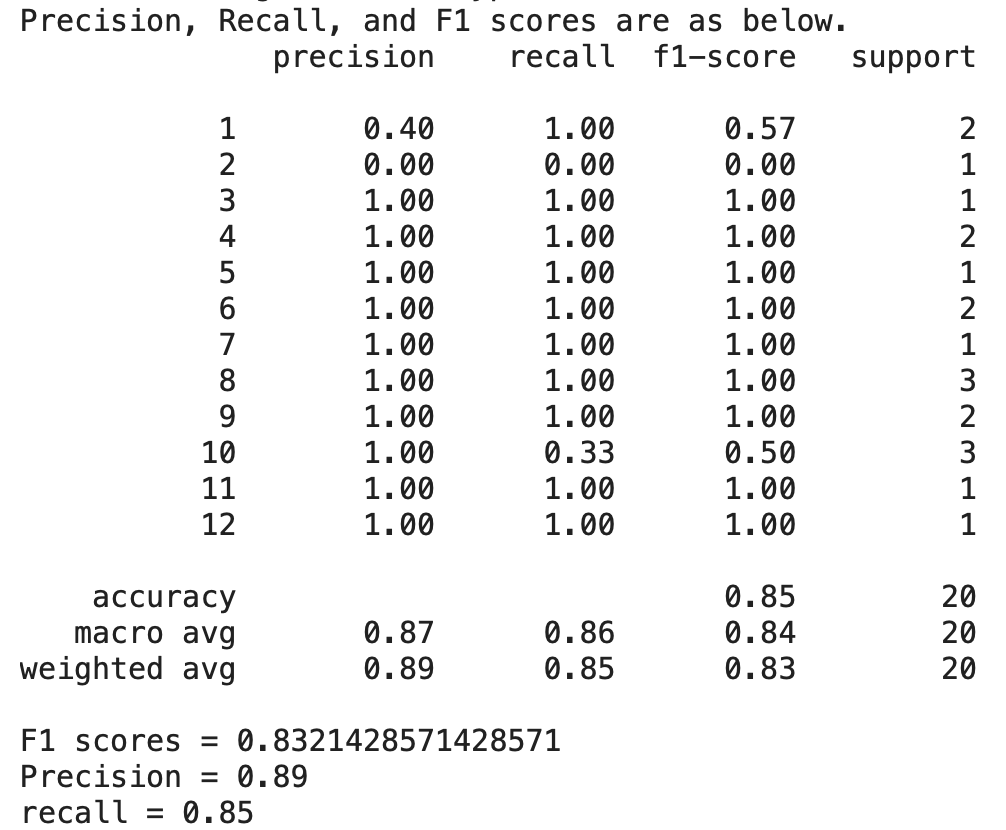
\includegraphics[width=10cm]{fig/nb_score.png}
    \caption{Precision, Recall, and F1 scores for Bernoulli Naïve Bayes method}
    \label{fig:galaxy}
\end{figure}

\begin{figure}[htp]
    \centering
    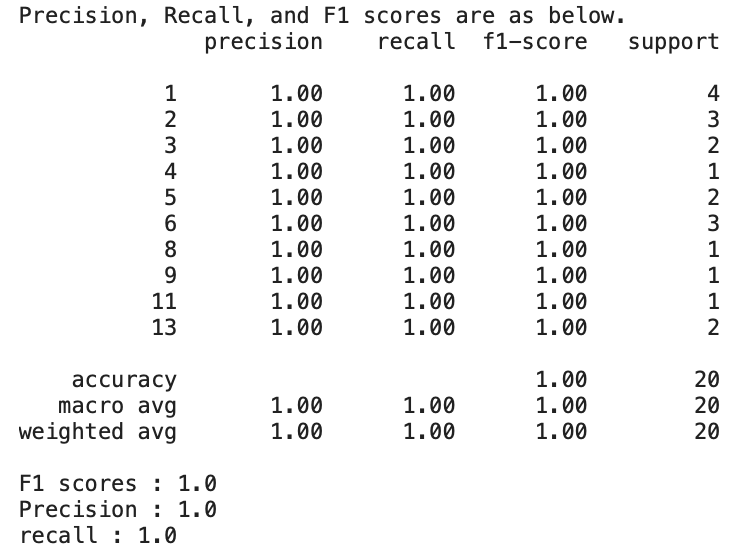
\includegraphics[width=10cm]{fig/svmL_score.png}
    \caption{Precision, Recall, and F1 scores for SVM method with linear kernel}
    \label{fig:galaxy}
\end{figure}

\begin{figure}[htp]
    \centering
    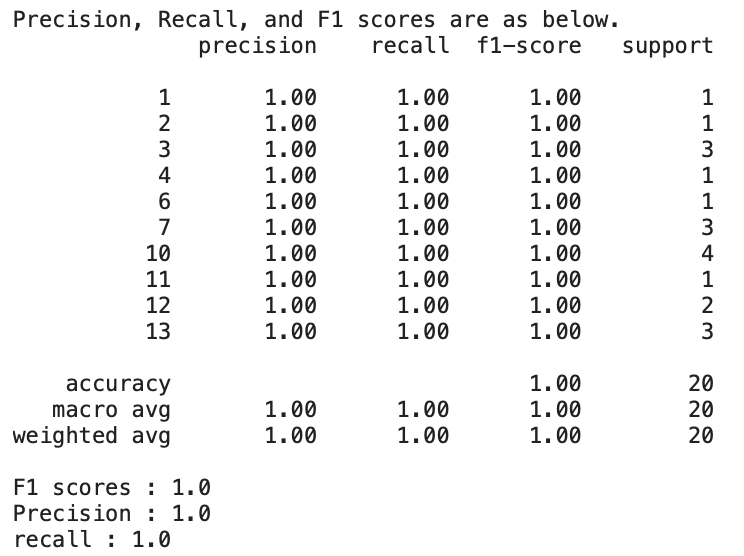
\includegraphics[width=10cm]{fig/svmR_score.png}
    \caption{Precision, Recall, and F1 scores for SVM method with RBF kernel}
    \label{fig:galaxy}
\end{figure}
\newpage
\section{Precision Recall Curves}
The precision recall curves for these three method are represented as below.
\begin{figure}[htp]
    \centering
    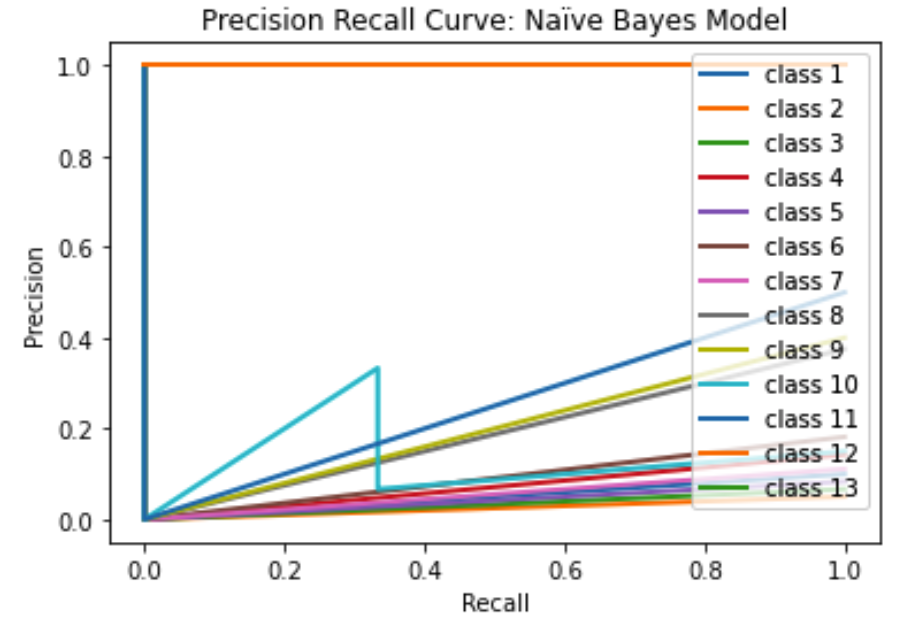
\includegraphics[width=10cm]{fig/nb_fig.png}
    \caption{Precision Recall curve for Bernoulli Naïve Bayes method}
    \label{fig:galaxy}
\end{figure}

\begin{figure}[htp]
    \centering
    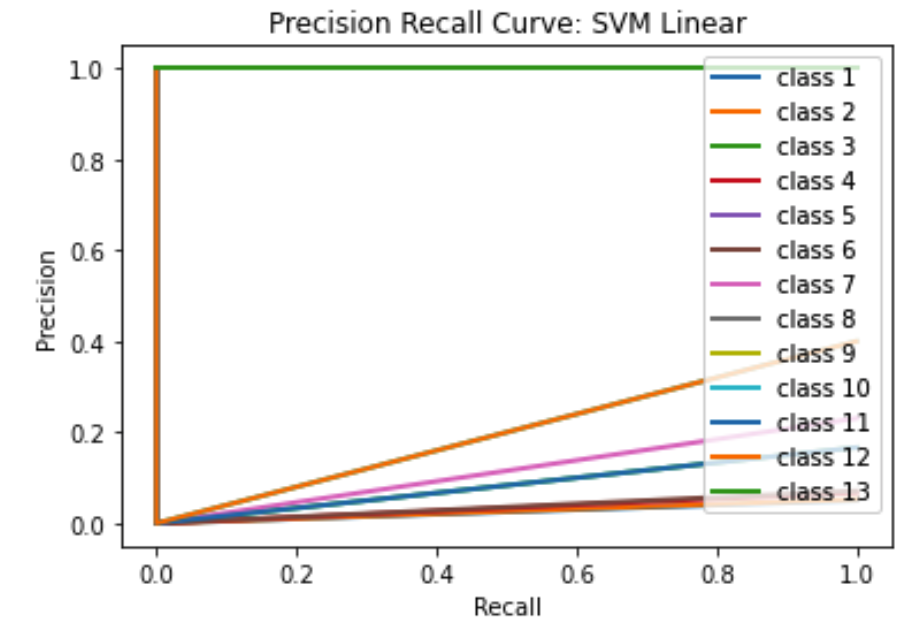
\includegraphics[width=10cm]{fig/svmL_fig.png}
    \caption{Precision Recall curve for SVM method with linear kernel}
    \label{fig:galaxy}
\end{figure}

\begin{figure}[htp]
    \centering
    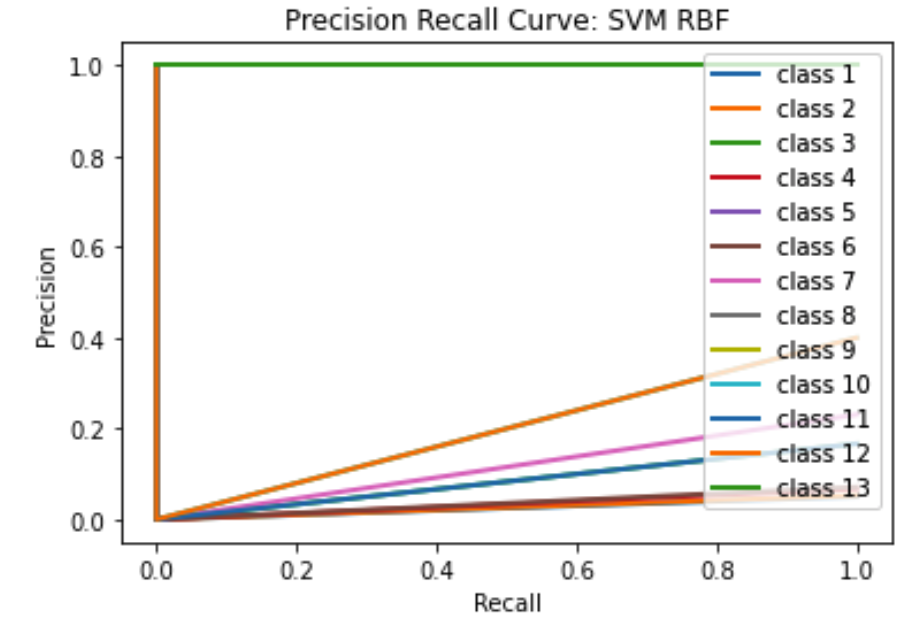
\includegraphics[width=10cm]{fig/svmR_fig.png}
    \caption{Precision Recall curve for SVM method with RBF kernel}
    \label{fig:galaxy}
\end{figure}
\newpage
\section{Scores on Kaggle}
The submission score on Kaggle is shown as below. I get 0.98444 on this competition, ranking at first place on Nov. 11th.
\begin{figure}[htp]
    \centering
    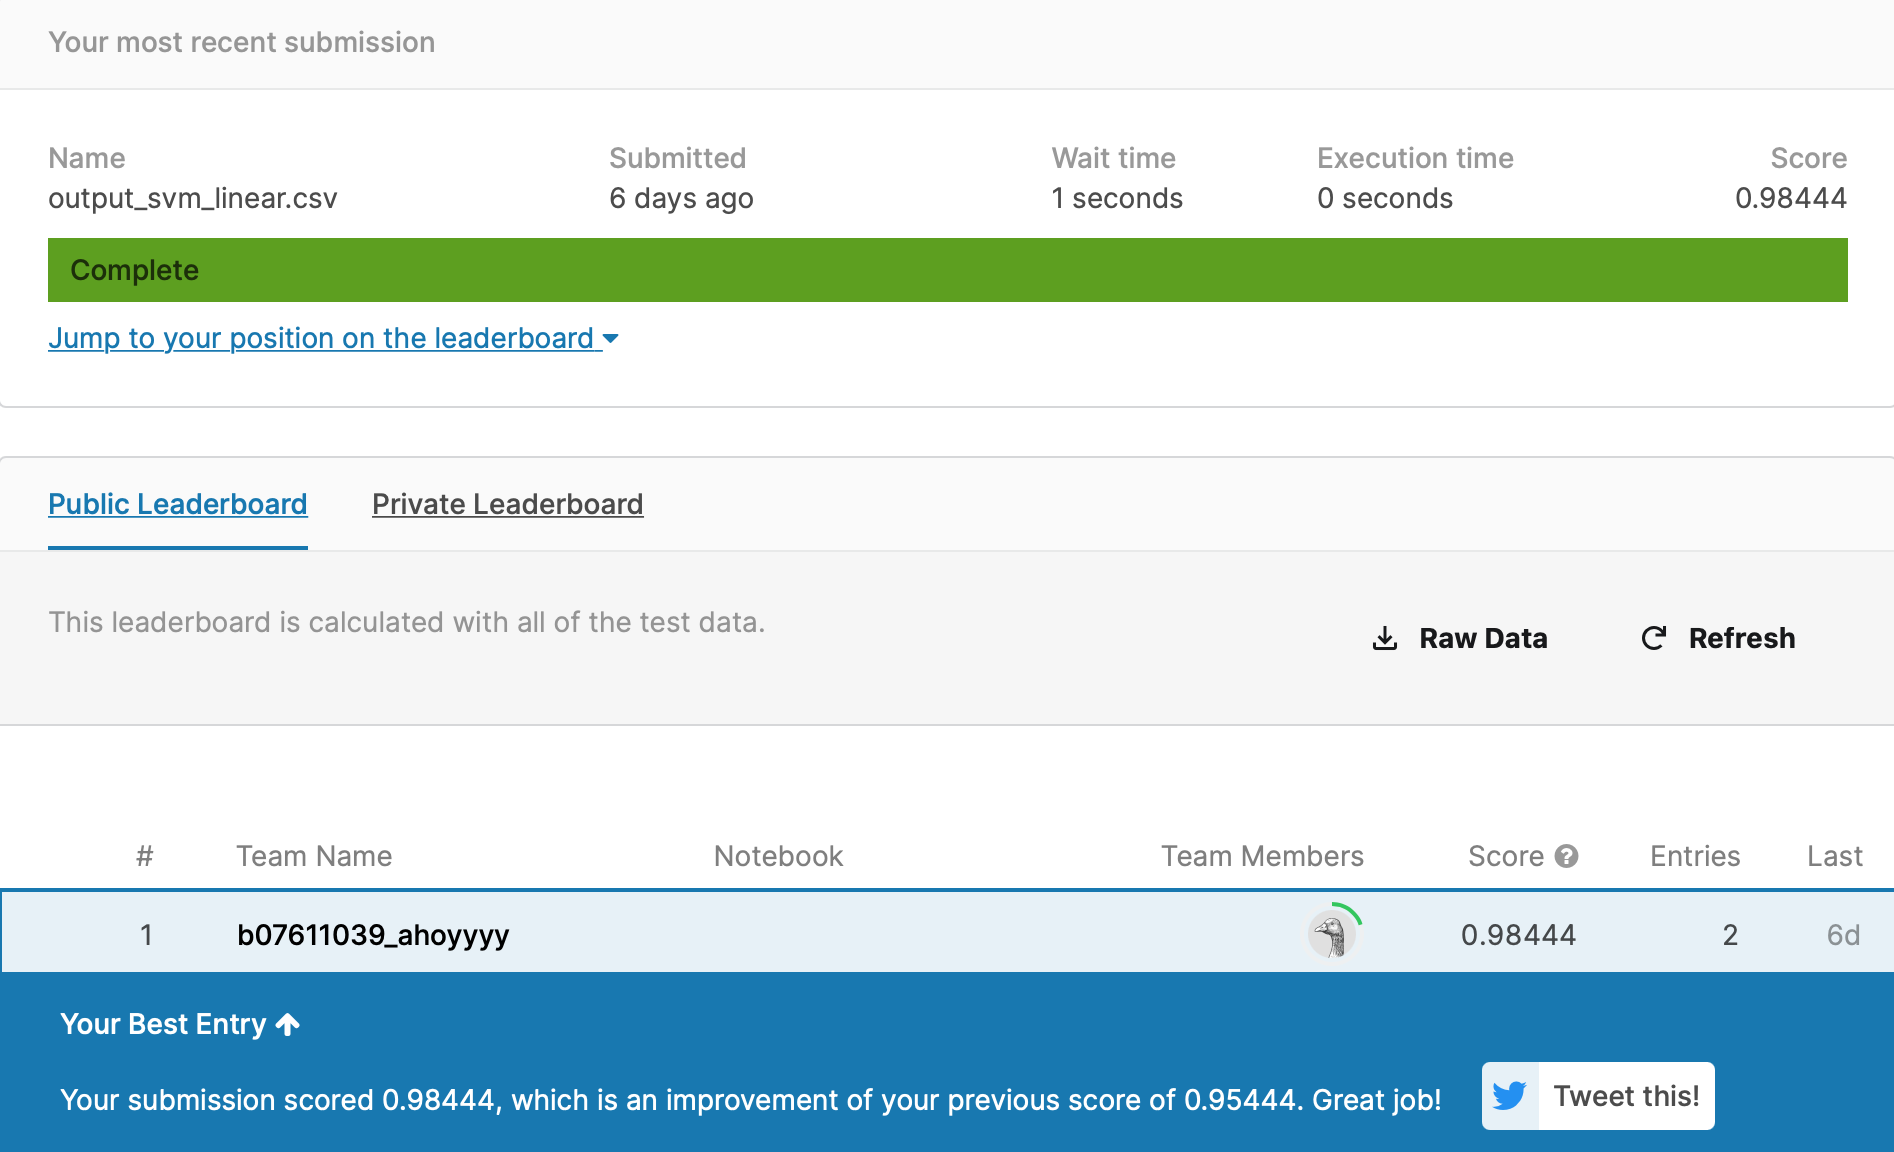
\includegraphics[width=10cm]{fig/scores}
    \caption{Score on Kaggle}
    \label{fig:galaxy}
\end{figure}

\section{Implement}
\subsection{Preprocess}
\begin{enumerate}
\item{
Import all necessary libraries, for example, sklearn, numpy, pandas, etc.
}
    \item{
Lowercase all words in docs, eliminate the stop word in English, replace EOL.
}
\item{
Separate the testing data set and the training data set.
\begin{lstlisting}[language=Python]
# classes stores the given testing data set via a 2D array
labels = []
for q in range(0, len(docs)):
    for i in range(0, 13):
        for j in range(0, 15):
            if q + 1 == classes[i][j]:
                labels.append([classes[i][j], i+1])
labels = pd.DataFrame(sorted(labels, key = lambda l:l[0]), columns = ['training_id', 'classes'])
training_docs = docs[docs['id'].isin(labels['training_id'])]
testing_docs = docs[~docs['id'].isin(labels['training_id'])]
\end{lstlisting}
}
\end{enumerate}

\subsection{Bernoulli Naïve Bayes}
\begin{lstlisting}[language=Python]
binary_vectorizer = CountVectorizer(binary = True)
binary_vectors = binary_vectorizer.fit_transform(training_docs['text'])
binary_vectors_test = binary_vectorizer.transform(testing_docs['text'])
x_train, x_test, y_train, y_test = train_test_split(binary_vectors, labels['classes'], test_size = 0.1) # amazing method taught by my classmates
model = BernoulliNB()
model.fit(x_train, y_train)
prediction = []
expectation = []
prediction.extend(model.predict(x_test))
expectation.extend(y_test)
\end{lstlisting}

\subsection{Linear Kernel SVM}
\begin{lstlisting}[language=Python]
TFIDF_vectorizer = TfidfVectorizer(stop_words = 'english')
TFIDF_vectors_training = TFIDF_vectorizer.fit_transform(training_docs['text'])
TFIDF_vectors_testing  = TFIDF_vectorizer.transform(testing_docs['text'])

x_train, x_test, y_train, y_test = train_test_split(TFIDF_vectors_training, labels['classes'], test_size = 0.1)
SVC_Linear_model = SVC(kernel='linear', C = 1.0)
SVC_Linear_model.fit(x_train, y_train)

prediction = []
expectation = []

prediction.extend(SVC_Linear_model.predict(x_test))
expectation.extend(y_test)
\end{lstlisting}

\subsection{RBF Kernel SVM}
\begin{lstlisting}[language=Python]
TFIDF_vectorizer = TfidfVectorizer(stop_words = 'english')
TFIDF_vectors_training = TFIDF_vectorizer.fit_transform(training_docs['text'])
TFIDF_vectors_testing  = TFIDF_vectorizer.transform(testing_docs['text'])

x_train, x_test, y_train, y_test = train_test_split(TFIDF_vectors_training, labels['classes'], test_size = 0.1)
SVC_RBF_model = SVC(kernel='RBF', C = 1.0)
SVC_RBF_model.fit(x_train, y_train)

prediction = []
expectation = []

prediction.extend(SVC_RBF_model.predict(x_test))
expectation.extend(y_test)
\end{lstlisting}


\newpage
\subsection{Representation of scores}
\begin{lstlisting}[language=Python]
print("Precision, Recall, and F1 scores are as below.")
print(metrics.classification_report(expectation, prediction))
print("F1 scores :", metrics.f1_score(expectation, prediction, average='weighted'))
print("Precision :", metrics.precision_score(expectation, prediction, average='weighted'))
print("recall :", metrics.recall_score(expectation, prediction, average ='weighted'))
\end{lstlisting}

\subsection{Plotting}
\begin{lstlisting}[language=Python]
precision = dict() 
recall = dict() 
for i in range(13):
    precision[i], recall[i], thresholds = metrics.precision_recall_curve(expectation, prediction, pos_label = (i + 1))
    plt.plot(recall[i], precision[i], lw = 2, label = 'class {}'.format(i + 1))

plt.xlabel("Recall") 
plt.ylabel("Precision")
plt.legend(loc = "upper right")
plt.title("Precision Recall Curve")
plt.show()
\end{lstlisting}


%\end{CJK*}
\end{document}

